\chapter{\ChapterTitleWorkOrganization}
\label{sec:organizacja-pracy}

W~tym rozdziale omówione zostały początkowe idee związane
z~formą i~funkcjami
aplikacji oraz zarysem harmonogramu działań.
Ponadto, zawiera informacje dotyczące przygotowania
narzędzi do weryfikacji postępu pracy, z~myślą o~osobach
nadzorujących proces
realizacji projektu.
Również przedstawiane
są narzędzia, które zespół wykorzystał do skutecznego
zarządzania
i~realizacji projektu. Opisana jest także struktura
organizacyjna
zespołu, jego role i~zadania w kontekście tworzenia
aplikacji.



\section{Charakterystyka i sposób realizacji projektu}

Najważniejsze wymogi dotyczące realizacji projektu
zostały określone na samym początku rozpoczęcia prac. Podzielono system na osobne elementy
mające spełniać odmienne zadania oraz rozrysowano wstępny plan długoterminowy. Przygotowano
również szkice interfejsu aplikacji. Plan prac był dostosowywany w~trakcie
kolejnych spotkań z~promotorem oraz
podczas rozmów z~klientem w~ramach zajęć pracowni projektowej.
Konsultacje te miały za zadanie nadanie najwyższego priorytetu
sprawom najważniejszym
dla udanej realizacji założeń projektu.

Realizacja projektu przyjęła ogólnie kaskadowy charakter --
ważne było, żeby powstawanie kolejnych części projektu nie było blokowane przez
brak elementów potrzebnych do ich działania. Z~tego powodu projekt był realizowany
etapami. Na początku napisano logikę gry w~brydża, ponieważ ustalono, że ta część
systemu powinna być już dobrze sprawdzona i~przetestowana przed powstaniem
aplikacji umożliwiającej rozgrywkę. Kolejnym etapem była realizacja funkcjonalności
związanych z~podstawowym interfejsem użytkownika, którego największą część
stanowiło lobby i~zarządzanie nim. Równoległe trwały prace nad serwerem gry, który
odpowiadał za utworzenie sesji między graczami i~przeprowadzenie między nimi rozgrywki.
Następnie rozpoczęto prace nad silnikiem gry, który
umożliwił użytkownikom wykonywanie ruchów. Ostatnim kamieniem milowym była implementacja
algorytmów odpowiadających za działanie wirtualnego asystenta oraz umożliwienie
wstawienia go jako gracza do rozgrywki z~użytkownikami.

Postawienie kamieni milowych było istotne w~celu weryfikowania postępów
nad projektem. Dzięki nim umożliwiono ustanowienie konkretnych celów oraz~przedstawienie
ich finalizacji klientowi i~osobom nadzorującym prace.

% TODO
% historia realizacji projektu
% co zostalo zlecone, jaki problem napotkalismy
% co zaplanowalismy, jak zaprojektowalismy
% cykl tworzenia
% milestone kluczowych funkcjonalnosci (lobby dziala, karty sa, mozna grac bez licytacji, wsyzstko dziala, dodany asystent)
% ogolne problemy i rozwiazania (bez szczegolow)
% mozna wspominac osoby za co odpowiadaly w danym czasie
% opisujemy z trzeciej osoby co robili tworzacy projekt
% i ich zadania (ogolnie bez szczegolow - wystarczy wspomniec dana konkretna czesc)
% ciekawe etapy ktore mialu duze znaczenie warto wspomniec


\section{Osoby w projekcie}

\subsection{Promotor}

Promotorem projektu był dr hab. inż. \textbf{Maciej Woźniak}, pracownik Instytutu Informatyki.
Po zapoznaniu się z~propozycją wykonania aplikacji umożliwiającej grę w~brydża ze sztuczną
inteligencją, przedstawioną przez członków zespołu projektowego, zgodził się on na zostanie
opiekunem pracy. Wykorzystując swoje doświadczenie w~pełnieniu tego stanowiska, w~trakcie regularnych
spotkań udzielał pomocnych porad dotyczących tworzenia aplikacji, ustalania kolejnych celów
i~tworzenia dokumentacji projektu.

\subsection{Zespół projektowy}
Przez sześć semestrów studiów inżynierskich na kierunku Informatyka, członkowie zespołu zdobywali
doświadczenie w~szeregu różnych zagadnień związanych z~tą dziedziną nauki, takich jak algorytmika,
rozwój aplikacji internetowych czy uczenie maszynowe. Dodatkowym celem projektu było doskonalenie
swoich umiejętności oraz zdobywanie nowych kompetencji. Dlatego oprócz sprawdzonych wcześniej technologii,
zespół zdecydował się eksperymentować także z~nowymi dla siebie narzędziami.
Skład zespołu i~ogólny podział obowiązków:
\begin{itemize}
    \item \textbf{Szymon Idec} -- implementacja logiki gry w brydża oraz silnika gry
    \item \textbf{Jakub Karbowski} -- rozwój serwera gry oraz algorytmów sztucznej inteligencji
          wykorzystywanych przez wirtualnego asystenta
    \item \textbf{Karol Śliwa} -- wygląd interfejsów aplikacji, funkcjonalności zarządzania stanem lobby
\end{itemize}
Podział ról w~projekcie nie był jednak rygorystyczny. Odpowiednio do potrzeb i~możliwości,
członkowie zespołu rozwijali różne części systemu. Jakub tworzył logikę komunikującą się z~serwerem po stronie
front-endu, Szymon rozwijał podstrony aplikacji, a~Karol dodawał obsługę niektórych akcji klienta także w~części
serwerowej. W~szczególności element Bridge Core wymagał wprowadzania zmian i~dodawania kolejnych testów
w~miarę rozwoju funkcjonalności rozgrywki oraz wirtualnego asystenta. Z~tego powodu wszyscy członkowie
zespołu dokonywali w~nim poprawek.


\section{Weryfikacja postępów w trakcie realizacji}

Sprawdzanie postępów stanowi nieodłączny element niemal każdego
projektu. Regularne ustalanie, co zostało już zrealizowane, jest kluczowe,
aby skutecznie wyznaczać nowe cele i~dostosowywać tempo prac.

%%% najpierw base, pozniej lobby, pozniej gra a na koncu gra z ai
%%% scisle powiazane z epicami

\subsection{Spotkania z promotorem}
Spotkania z~promotorem odbywały się przeważnie co dwa tygodnie, choć ich częstotliwość
ulegała zmianom zgodnie z~bieżącymi potrzebami i~możliwościami. Na końcowym etapie realizacji projektu zdecydowano
się na spotkania cotygodniowe, ponieważ z~uwagi na stopień zaawansowania prac konieczność odbywania
konsultacji była większa. Spotkania prowadzono stacjonarnie oraz przy użyciu platformy Microsoft Teams.

\subsection{Pracownia projektowa}
Zajęcia pracowni projektowej miały miejsce raz w~tygodniu, natomiast na szczegółowe konsultacje
poszczególne grupy umawiały się z~prowadzącym pracownię indywidualnie. Większość spotkań miała
miejsce stacjonarnie w~budynku uczelni, jednak w~przypadkach, kiedy było to utrudnione, korzystano
z~Microsoft Teams.

%%% to opisujmey w obu przypadkach \subsubsection{Microsoft Teams}


\section{Wykorzystywane narzędzia do realizacji i organizacji pracy}

Do realizacji projektu zostało wykorzystane wiele narzędzi i~technologii
dostępnych za darmo lub jako produkty open source, czyli takie,
których właściciel praw autorskich przyznaje użytkownikom prawa
do swobodnego używania, modyfikacji i~udostępniania oprogramowania.
Było to kluczowe, aby zastosowane narzędzia i~technologie pozwoliły
na utworzenie darmowego rozwiązania. Dzięki temu użytkownicy
mogą sami uruchomić cały system, aplikację wraz z~wirtualnym
asystentem, bez posiadania płatnych licencji.


\subsection{Planowanie i projektowanie}

Przed rozpoczęciem tworzenia pierwszego kodu aplikacji niezbędne było
opracowanie ogólnego planu i~pierwotnej wizji projektu. Zdecydowano
się na przygotowaniu strategii działania oraz
zarysu celów i~funkcji, które mają być zrealizowane w~ramach projektu.
To etap planowania stanowił fundament dla późniejszej implementacji
i~umożliwił efektywne kierowanie procesem tworzenia aplikacji.

Co więcej, w~ramach tego wstępnego etapu, zwrócono uwagę na
opracowanie wizualizacji aplikacji. Starano się osiągnąć jasny
zarys wyglądu aplikacji webowej poprzez stworzenie wstępnych projektów
interfejsu użytkownika. Ta wizualizacja odegrała kluczową rolę
w~procesie projektowania, umożliwiając zespołowi uzyskanie wyobrażenia
o~finalnym wyglądzie aplikacji i~jednocześnie dostosowywanie projektu
do oczekiwań i~potrzeb użytkowników, jak i~wzorowaniu się na utworzonej
wizualizacji.


\subsubsection{Shortcut}

Praktycznie zawsze w~trakcie tworzenia oprogramowania wymagane jest
narzędzie lub platforma udostępniająca możliwość tworzenia zadań,
zależności między nimi oraz dzielenia na większe zbiory zadań.

\begin{figure}[h!]
    \centering
    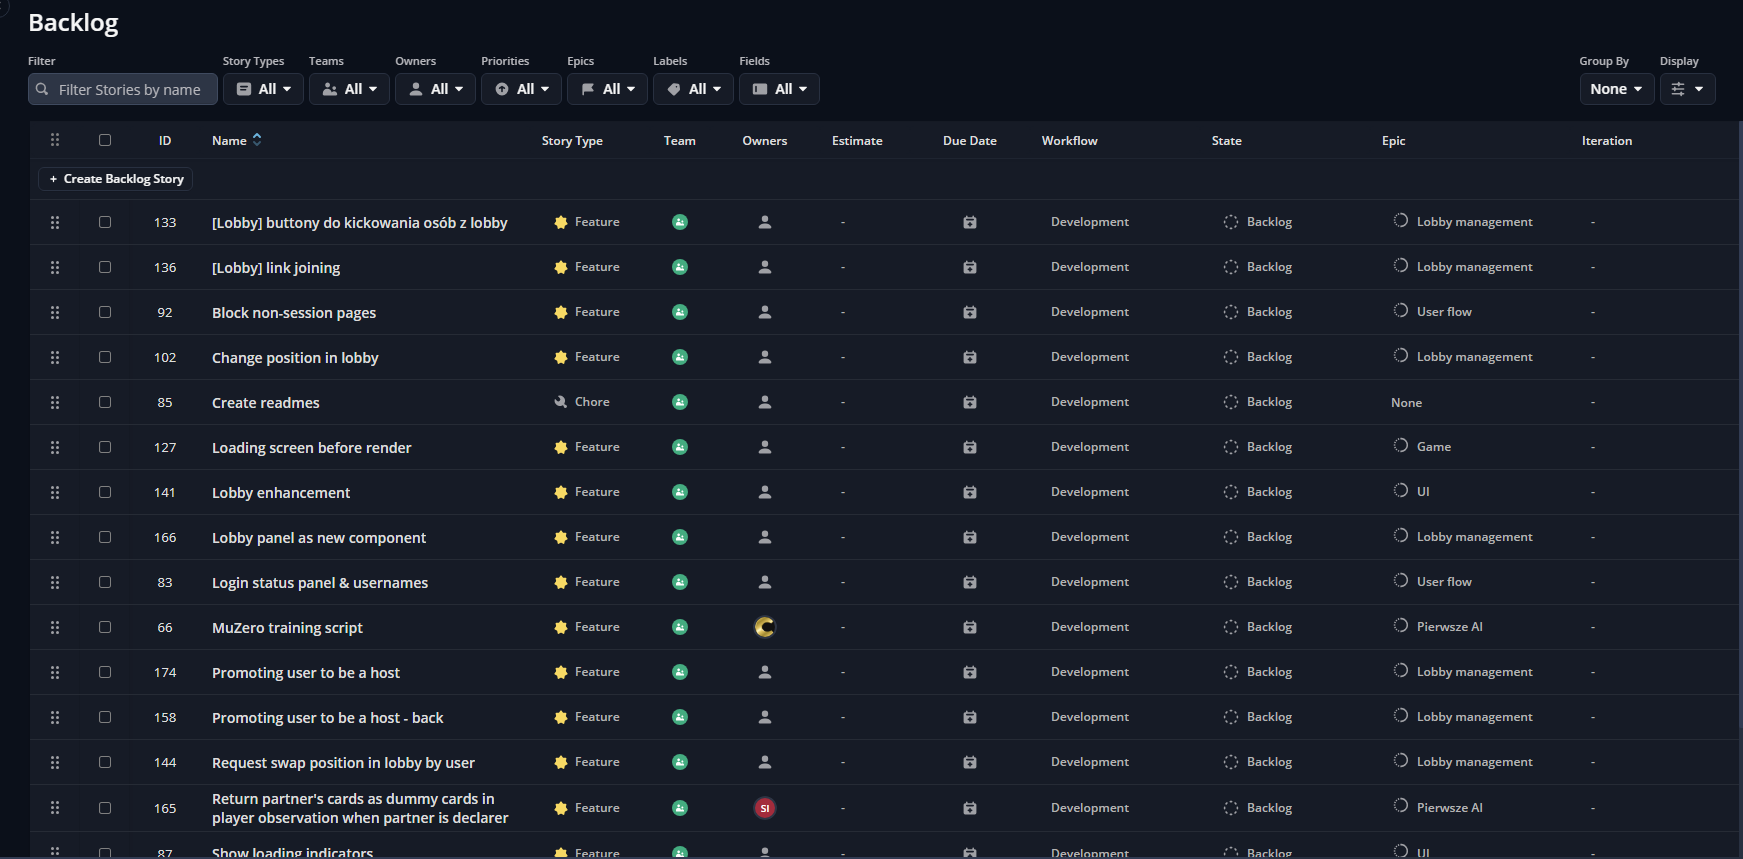
\includegraphics[width=0.9\textwidth]{img/shortcut/shortcut_backlog.png}
    \caption{Backlog z zadaniami}
    \label{fig:xd_shortcut_backlog}
\end{figure}

\begin{figure}[h!]
    \centering
    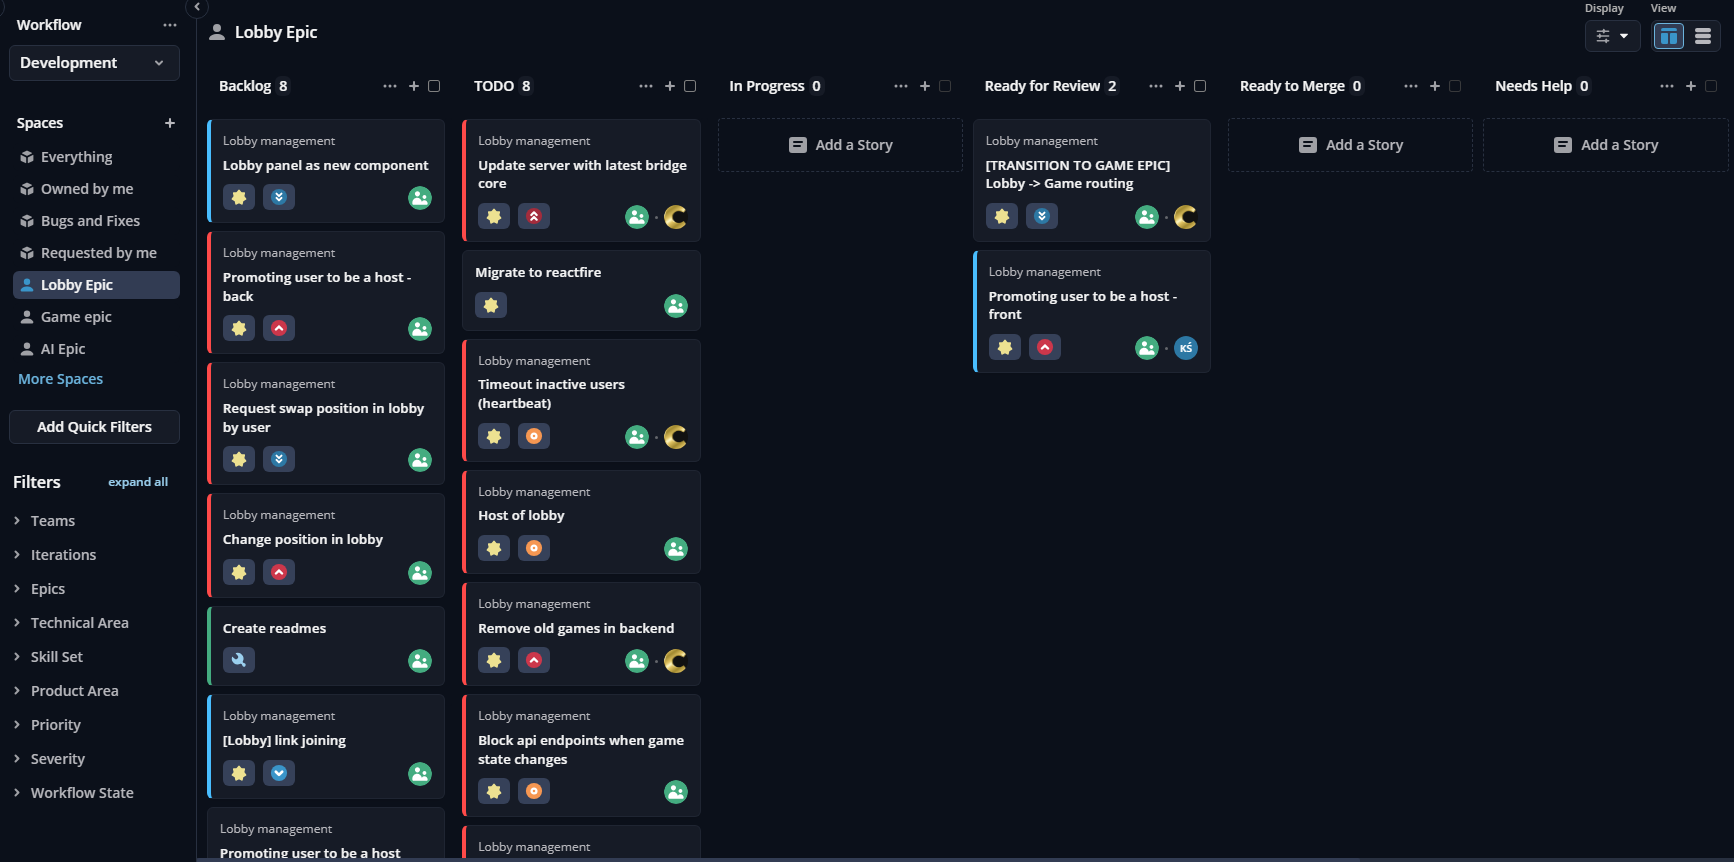
\includegraphics[width=0.9\textwidth]{img/shortcut/shortcut_epic.png}
    \caption{Epic dotyczący systemu lobby wraz z~zadaniami i~ich statusami}
    \label{fig:xd_shortcut_epic}
\end{figure}

Zdecydowano się na narzędzie Shortcut
\cite{Shortcut} (Rys.~\ref{fig:xd_shortcut_backlog}, \ref{fig:xd_shortcut_epic}),
które oferuje
wszystkie potrzebne funkcjonalności. Pozwala na podział zadań na tzw.
epiki -- elementy pracy zawierające wystarczająco dużo zadań do realizacji,
których nie da się ukończyć w~krótkim czasie. Dla każdego kamienia milowego
utworzono odpowiedni epik, dzięki czemu możliwe było prezentowanie
kolejnych części i~kluczowych etapów procesu tworzenia aplikacji.

\FloatBarrier

Również dużym plusem tego rozwiązania była integracja
z~platformą GitHub~\cite{Github}, która pozwoliła na
szybkie wyszukiwanie zmian w~kodzie projektu. Poprzez
zastosowane unikalnych identyfikatorów każde zadanie
znajdujące się w~Shortcut mogło mieć odpowiednio przypisaną
zmianę, która zaszła w~projekcie.


\subsubsection{Figma}

Do utworzenia wstępnej wizualizacji aplikacji użyto narzędzie Figma \cite{Figma}.
Służy ono do projektowania graficznego, takich prac jak szkielety stron
internetowych, prototypy interfejsów użytkownika czy też otwartych przestrzeni
do zarządzania i~planowania.

Warto wspomnieć, że tak jak w~\ref{fig:figma_login} lub
\ref{fig:figma_userflow} wykorzystano Figmę do stworzenia mocków i~schematów.

\FloatBarrier

\subsection{Komunikacja wewnętrzna}

W~trakcie tworzenia projektu potrzebna była szybka i~efektywna
wymiana wiadomości oraz możliwość współpracy w czasie rzeczywistym.
Wykorzystana została w~tym celu platforma Discord~\cite{Discord},
która oferuje rozmowy głosowe, kanały tekstowe i~udostępnianie
obrazu na żywo.


\subsection{System kontroli wersji}

Aby synchronizować postępy pracy i~ich historię zastosowano
system kontroli wersji Git~\cite{Git}. Wraz z~nim, do przechowywania
repozytoriów z kodem aplikacji, jak i~dokumentacji wykorzystano
platformę GitHub \cite{Github}.


\subsection{Tworzenie oprogramowania}

Rozwój oprogramowania stanowił kluczowy i~niezbędny element realizacji
założeń projektowych.
Celem było stworzenie funkcjonalnej aplikacji, która integruje
odmienne komponenty, wykorzystujące różne technologie.
W~tym celu skorzystano z~różnych narzędzi, które specjalizowały się
w~tworzeniu i~testowaniu oprogramowania, w~wymaganych przez projekt
technologiach.


\subsubsection{VSCode}

Visual Studio Code~\cite{VSCode}, dalej opisywany jako VSCode,
to zaawansowany edytor kodu stworzony
przez Microsoft, który stał się jednym z~najpopularniejszych narzędzi
wśród programistów~\cite{IDEIndex}.
VSCode wspiera wiele języków programowania i~znaczników od JavaScript,
TypeScript, Python, C++, Rust po HTML, CSS, JSON i~wiele innych.
Dużą zaletą VSCode jest również możliwość personalizacji. Dostępne są
tysiące rozszerzeń, które pozwalają na dostosowanie edytora do własnych
potrzeb. Użycie tego edytora znacznie usprawniło rozwój aplikacji.

Ze względu na możliwość dostosowania go do różnych języków programowania
i~technologii, stosowano go przy tworzeniu każdego elementu projektu.

Oprócz tworzenia w~tym narzędziu systemu brydża wykorzystano go także
do stworzenia dokumentacji aplikacji wraz z~użyciem systemu kontroli wersji Git.
Usprawniło to przebieg pracy nad dokumentem, jak i~wzajemną kontrolę
współtworzenia tekstu.


\subsubsection{Produkty Jetbrains}

Produkty JetBrains \cite{JetBrains}, w~tym dedykowane środowiska
programistyczne (IDE) dla poszczególnych języków i~ekosystemów,
takich jak Java, Python czy PHP, oferują zaawansowane funkcje
autouzupełniania i~głębokiej
analizy kodu. Dostarczają one również narzędzia do refaktoryzacji,
co znacząco ułatwia zarządzanie i~optymalizację projektu.

PyCharm \cite{PyCharm}, specjalizujący się w~Pythonie, był pomocny podczas tworzenia
modułu logiki gry w~brydża, a~także w~początkowej fazie konstruowania
serwera z~użyciem FastAPI.

Z~kolei IntelliJ IDEA \cite{Intellij}, ze wsparciem dla języka
Scala, znalazł zastosowanie w~procesie rozwijania ostatecznej wersji
architektury serwerowej.


\subsubsection{Postman}

Postman \cite{Postman} to narzędzie do testowania API, które umożliwia, głównie
programistom i testerom, skuteczne zarządzanie, tworzenie, udostępnianie
i~testowanie żądań HTTP. Jest to popularne środowisko do tworzenia
i~wykonywania zapytań HTTP, zwłaszcza w~kontekście testowania
endpointów RESTful API.

Postman oferuje intuicyjny interfejs graficzny, który ułatwia tworzenie,
wysyłanie i~analizowanie komunikatów sieciowych, a~także sprawdzanie
odpowiedzi serwera. Przydaje się w~wielu etapach procesu tworzenia
aplikacji, od projektowania, wczesnego testowania i~monitorowania API
w~środowisku produkcyjnym.

Przez cały proces tworzenia serwera dla aplikacji Postman był wykorzystywany
do wspomnianych wyżej celów. Było to narzędzie kluczowe w~zapewnieniu
poprawności działania tej części systemu.


\subsection{Integracja elementów systemu}

Podział tworzonego systemu na wiele części
takich jak aplikacja webowa, serwer, wirtualny asystent
i~dokumentacja wymagał stworzenia odpowiedniego
przepływu pracy zwanego \mbox{\textbf{CI/CD}}. Akronim ten oznacza
ciągłą integrację/ciągłe wdrażanie. Jest on stosowany
w~celu szybkiego likwidowania błędów, przeprowadzania
testów, analizą działania i~integracją elementów systemu
aplikacji. Również pozwala on przyrostowe implementowanie
projektu i~możliwość otrzymania od klienta zwrotnych
informacji o~działaniu systemu.

Zastosowanie tego rozwiązania pozwoliło na
prezentowanie klientowi kolejnych etapów aplikacji, jak
również pozwoliło na niezależne rozwijanie
i~testowanie osobnych części systemu.

Poniżej opisano technologie i~zaprojektowane systemy,
które pozwoliły na skonstruowanie systemu CI/CD dla
tworzonego projektu.


\subsubsection{Github Actions}

Najważniejszym elementem całego systemu było zintegrowanie
repozytorium kodu
wraz z~resztą technologii. Platforma GitHub, na której
znajduje się kod tworzonej aplikacji, oferuje swoje
rozwiązanie GitHub Actions~\cite{GithubActions} pozwalające
na zaawansowaną realizację CI/CD. Dla każdego elementu
projektu zostały utworzone instrukcje w~postaci plików JSON
lub wykorzystano integracje zewnętrznych narzędzi oferujące
automatyczne konfiguracje. Instrukcje te były uruchamiane
po aktualizacji kodu.


\subsubsection{Vercel}

\begin{figure}[!]
    \centering
    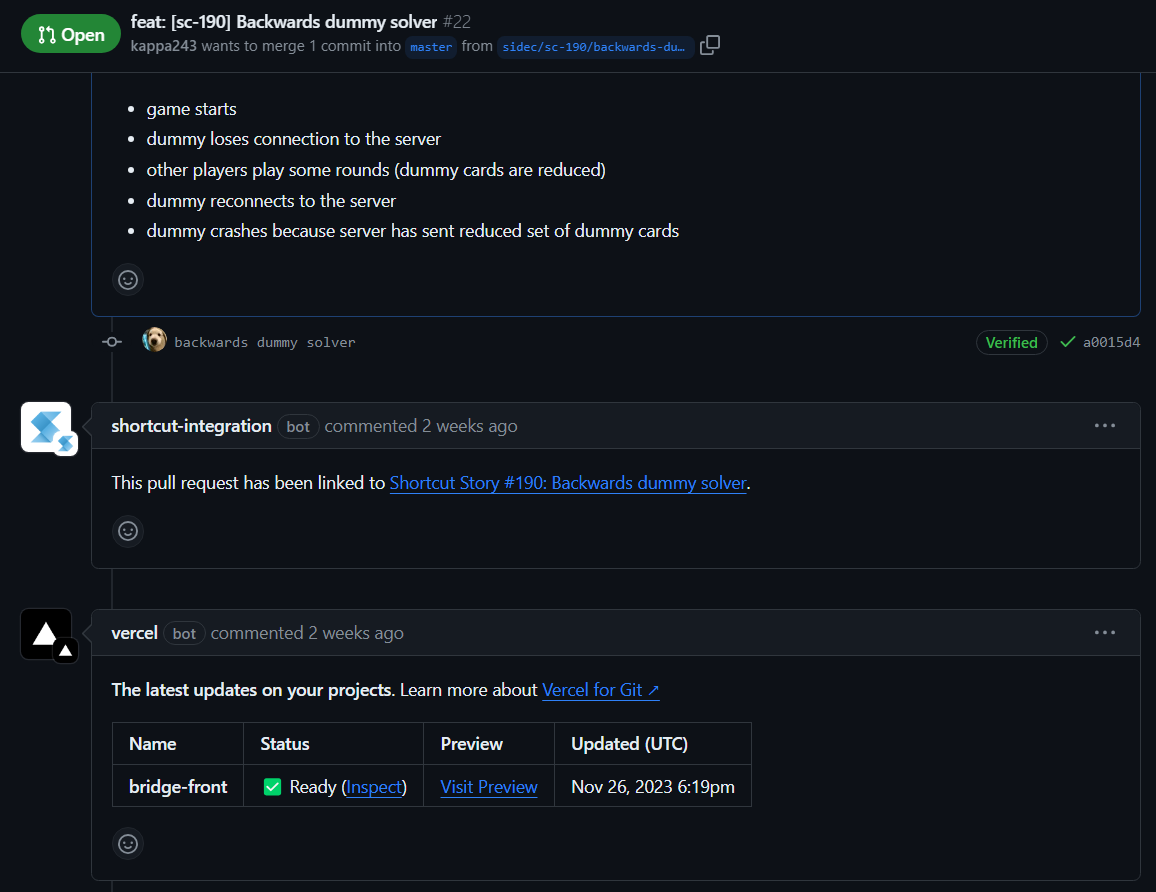
\includegraphics[width=0.9\textwidth]{img/github/github-vercel.png}
    \caption{Wycinek integracji platformy Vercel z~GitHub dla jednej z~gałęzi kodu aplikacji webowej}
    \label{fig:github-vercel}
\end{figure}

Platforma Vercel była odpowiedzialna za
udostępnianie aplikacji webowej. Posiada ona wsparcie \mbox{z~GitHubem},
przez co tworzenie instrukcji odbywa się automatycznie.
Vercel, dla głównej gałęzi kodu "\textit{master}"\xspace oraz
gałęzi implementujących dodatkowe funkcje, budował aplikację
i~udostępniał na swojej platformie. W~przypadku aktualizacji
kodu, na odpowiednich gałęziach, przystępował on do ponownego
budowania aplikacji i~zastępował starą. Dla każdej gałęzi
generowany był osobny adres, więc w~przypadku zmian zawsze
najnowsza wersja aplikacji, z~danej gałęzi, była dostępna pod
tym samem odpowiadającym jej adresem. Co więcej, w przypadku
problemów lub błędów podczas budowania aplikacji, informuje
on o~tym i~udostępnienia zapisy logów, aby można było je
zweryfikować.

Na rysunku
\ref{fig:github-vercel} można zauważyć, jak dla jednej
z~gałęzi został wygenerowany adres do aplikacji
("Visit Preview") oraz że budowanie przebiegło bez problemów
(zielone zaznaczenie).

\FloatBarrier


\subsubsection{Oracle Cloud}

\begin{figure}[!]
    \centering
    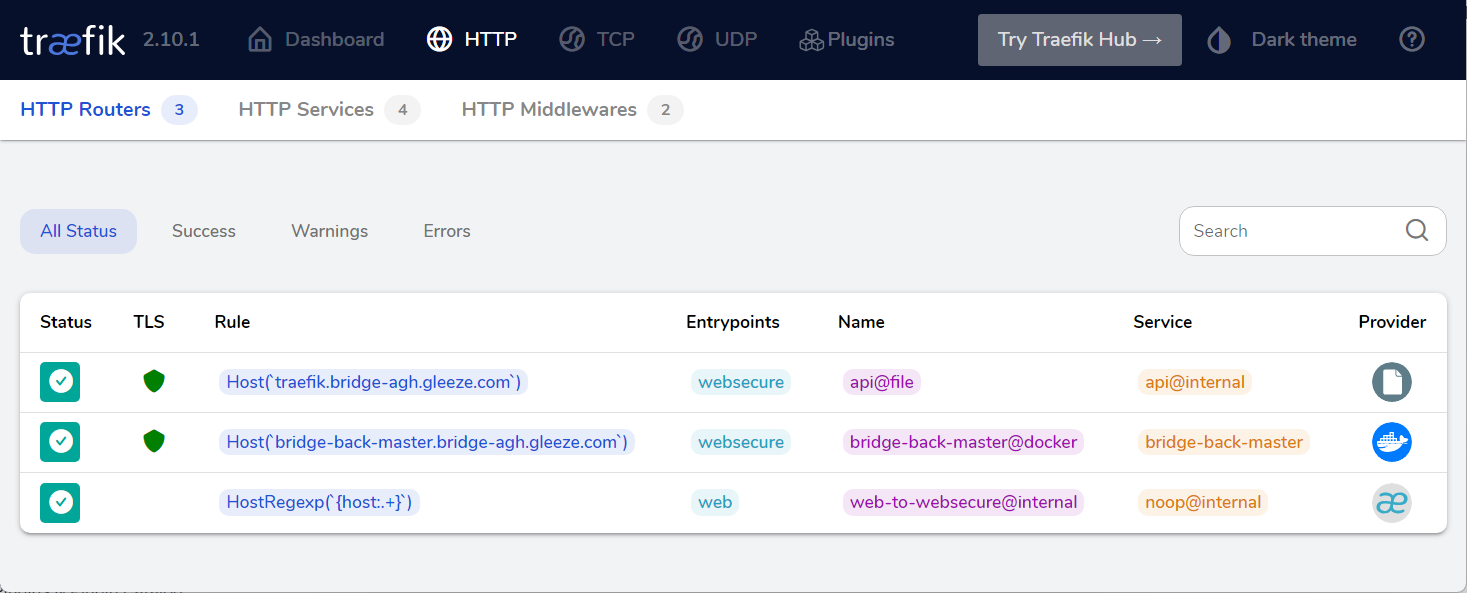
\includegraphics[width=0.9\textwidth]{img/traefik/dashboard.png}
    \caption{Panel serwisów udostępnionych przez Traefik.}
    \label{fig:traefik-dashboard}
\end{figure}

Do uruchomienia serwera naszego systemu wymagane było
osobne środowisko, w~którym możemy uruchomić
narzędzie do automatycznego budowania i~udostępniania
najnowszych wersji serwera, w~podobny sposób jak zostało
to rozwiązane w~przypadku aplikacji webowej.

Zrealizowano takie rozwiązanie poprzez stworzenie autorskiego
narzędzia wraz z~wykorzystaniem serwera udostępnionego
przez platformę Oracle Cloud.
Wykorzystując możliwość tworzenia instrukcji GitHub Actions
skonfigurowano automatyczne tworzenie obrazu kontenera
Docker~\cite{Docker}, który miał za zadanie uruchamiać
serwer gry. Utworzony kontener był udostępniany w~rejestrze
przechowujących takie obrazy na
platformie GitHub. Następnie po stronie serwera Oracle
cyklicznie sprawdzany był rejestr w~celu wykrycia
nowo powstałego obrazu kontenera. Gdy obraz posiadał
inny hash\footnote{hash -- wartość wyliczana przez tzw. "funkcję
    hashującą", która dla otrzymanych na wejściu tych
    samych danych zwraca tę samą wyliczoną wartość.}
odpowiedni skrypt uruchamiał nową wersję kontenera.
Każda gałąź kodu, podobnie jak w~przypadku aplikacji
webowej, posiadała osobny kontener uruchomiony na serwerze
Oracle, do którego tworzony był osobny adres za pomocą
utworzonych skryptów i~oprogramowania Traefik~\cite{Traefik} (Rys.~\ref{fig:traefik-dashboard}).
Dzięki temu aplikację webową można było połączyć
z~dowolnie wybraną wersją serwera gry, na przykład, aby
przetestować nową funkcjonalność. Na rysunku
\ref{fig:traefik-dashboard} przedstawiono panel, na którym
znajduje się lista serwerów udostępnionych dla
odpowiadających im gałęzi kodu.

\FloatBarrier


\subsection{Testowanie oprogramowania}

Najważniejszym w~kontekście działania całego systemu
było zapewnienie prawidłowego funkcjonowania
serwera gry, logiki gry brydża i~asystenta.
Jest to bardzo istotne w~procesie tworzenia oprogramowania,
który opiera się na ciągłym dodawaniem kolejnych
funkcjonalności, gdyż każdy dodany element może doprowadzić
do wadliwego działania poprzez najdrobniejszy błąd.

Aby zapobiec takim zdarzeniom, zdecydowano się na utworzenie
testów, które obejmowały znaczną część kodu w~wymienionych
wyżej elementach aplikacji. Przy aktualizacji kodu,
podobnie jak we wspomnianym wcześniej systemie integracji,
testy były uruchamiane automatycznie. Podczas wystąpienia
błędu na platformie GitHub widoczna jest informacja
o~nieudanym przeprowadzeniu testów
(Rys. \ref{fig:github-commits}, \ref{fig:github-tests}).

\begin{figure}[hbt!]
    \centering
    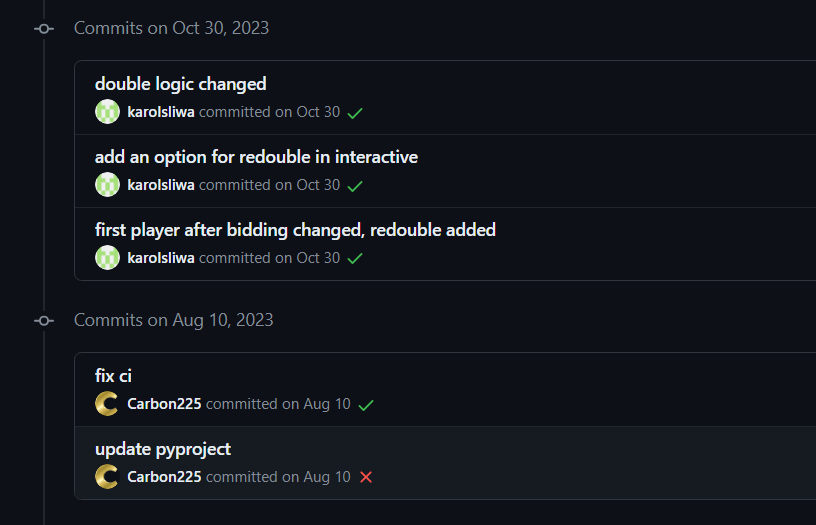
\includegraphics[width=0.9\textwidth]{img/github/github-commits.png}
    \caption{Lista commitów z informacją o przebiegu testów dla Bridge Core}
    \label{fig:github-commits}
\end{figure}

\begin{figure}[hbt!]
    \centering
    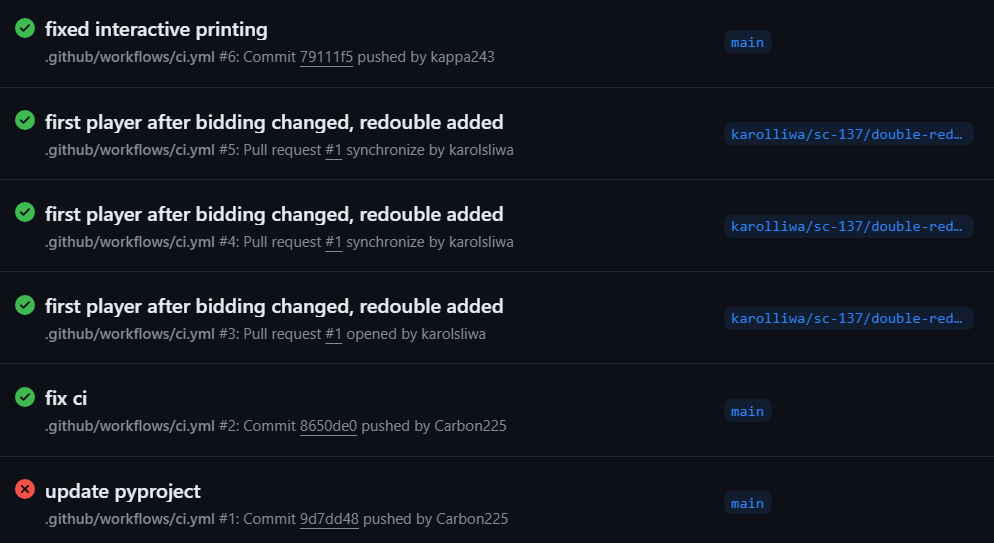
\includegraphics[width=0.9\textwidth]{img/github/github-tests.png}
    \caption{Lista uruchomionych testów przez GitHub Actions dla Bridge Core}
    \label{fig:github-tests}
\end{figure}


\subsection{Tworzenie dokumentacji}

Do napisania dokumentacji aplikacji użyto języka \LaTeX~\cite{Latex}.
Przesyłając zmiany w~tekście pracy na platformę GitHub, za pomocą
GitHub Actions, generowano natychmiastowo dokument PDF.
Umożliwiło to na dostęp do najnowszej wersji dokumentu dla opiekuna
pracy i~prowadzącego pracownię projektową, dzięki czemu była możliwa
ciągła weryfikacja postępów nad pracą.

